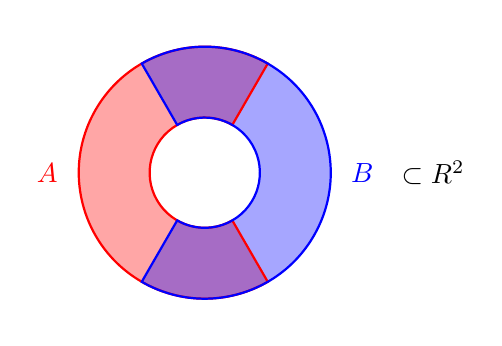
\begin{tikzpicture}
\fill[red, opacity=0.35] (60:1.6) arc[start angle=60, end angle=300, radius=1.6] -- (300:0.7) arc[start angle=300, end angle=60, radius=0.7] -- cycle;
\fill[blue, opacity=0.35] (-120:1.6) arc[start angle=-120, end angle=120, radius=1.6] -- (120:0.7) arc[start angle=120, end angle=-120, radius=0.7] -- cycle;
\draw[red, thick] (60:1.6) arc[start angle=60, end angle=300, radius=1.6] -- (300:0.7) arc[start angle=300, end angle=60, radius=0.7] -- cycle;
\draw[blue, thick] (-120:1.6) arc[start angle=-120, end angle=120, radius=1.6] -- (120:0.7) arc[start angle=120, end angle=-120, radius=0.7] -- cycle;
\node[red] at (180:2.0) {$A$};
\node[blue] at (0:2.0) {$B$};
\node at (2.9,0) {$\subset \mathbb{R}^2$};
\end{tikzpicture}
